\documentclass[twocolumn,useAMS,usenatbib]{mn2e}
%\usepackage{natbib}
\usepackage{amsmath}
%\usepackage{amssymb}
\usepackage{latexsym}
\usepackage{epsfig,graphicx}
\usepackage{subfig}
\usepackage{float}
\topmargin-1cm

% For correct printing on US Letter, while still working on A4
\topmargin-1cm

\def\a{\alpha}
\def\reff@jnl#1{{\rm#1\/}}

\def\aj{\reff@jnl{AJ}}                  % Astronomical Journal
\def\araa{\reff@jnl{ARA\&A}}            % Annual Review of Astron and Astrophys
\def\apj{\reff@jnl{ApJ}}                        % Astrophysical Journal
\def\apjl{\reff@jnl{ApJ}}               % Astrophysical Journal, Letters
\def\apjs{\reff@jnl{ApJS}}              % Astrophysical Journal, Supplement
\def\apss{\reff@jnl{Ap\&SS}}            % Astrophysics and Space Science
\def\aap{\reff@jnl{A\&A}}               % Astronomy and Astrophysics
\def\aapr{\reff@jnl{A\&A~Rev.}}         % Astronomy and Astrophysics Reviews
\def\aaps{\reff@jnl{A\&AS}}             % Astronomy and Astrophysics, Supplement
\def\baas{\reff@jnl{BAAS}}              % Bulletin of the AAS
\def\jrasc{\reff@jnl{JRASC}}            % Journal of the RAS of Canada
\def\memras{\reff@jnl{MmRAS}}           % Memoirs of the RAS
\def\mnras{\reff@jnl{MNRAS}}            % Monthly Notices of the RAS
\def\physrep{\reff@jnl{Phys.Rep.}}
\def\pra{\reff@jnl{Phys.Rev.A}}         % Physical Review A: General Physics
\def\prb{\reff@jnl{Phys.Rev.B}}         % Physical Review B: Solid State
\def\prc{\reff@jnl{Phys.Rev.C}}         % Physical Review C
\def\prd{\reff@jnl{Phys.Rev.D}}         % Physical Review D
\def\prl{\reff@jnl{Phys.Rev.Lett}}      % Physical Review Letters
\def\pasp{\reff@jnl{PASP}}              % Publications of the ASP
\def\pasj{\reff@jnl{PASJ}}              % Publications of the ASJ
\def\skytel{\reff@jnl{S\&T}}            % Sky and Telescope
\def\solphys{\reff@jnl{Solar~Phys.}}    % Solar Physics
\def\sovast{\reff@jnl{Soviet~Ast.}}     % Soviet Astronomy
\def\ssr{\reff@jnl{Space~Sci.Rev.}}     % Space Science Reviews
\def\nat{\reff@jnl{Nature}}             % Nature

\def\sun{\hbox{$\odot$}}
\def\farcs{\hbox{$.\!\!^{\prime\prime}$}}
\newcommand{\hvol}{h^{3}{\mathrm{Mpc}}^{-3}}
\newcommand{\hmpc}{\ensuremath{h^{-1}\mathrm{Mpc}}}
\newcommand{\hkpc}{\ensuremath{h^{-1}\mathrm{kpc}}}
\newcommand{\hMsun}{h^{-1}M_{\odot}}
\newcommand{\Msun}{M_{\odot}}
\newcommand{\kms}{{\,{\rm km}\,{\rm s}^{-1}}}
\newcommand{\Omegam}{\Omega_{m}}
\newcommand{\Omegab}{\Omega_{b}}
\newcommand{\Omegal}{\Omega_{\Lambda}}
\newcommand{\xig}{\xi_{\rm gg}(r)}
\newcommand{\xih}{\xi_{\rm hh}(r)}
\newcommand{\xim}{\xi_{\rm mm}(r)}
\newcommand{\ds}{\ensuremath{\Delta\Sigma}}
\newcommand{\scinv}{\ensuremath{\Sigma_c^{-1}}}
\newcommand{\avgscinv}{\ensuremath{\langle\Sigma_c^{-1}\rangle}}
\newcommand{\hinvk}{$h^{-1}$kpc}
\newcommand{\avgnm}{\ensuremath{\langle N(M)\rangle}}
\newcommand{\fclust}{\ensuremath{f_\mathrm{clust}}}
\newcommand{\fbcg}{\ensuremath{f_\mathrm{BCG}}}

\newcommand{\beq}{\begin{equation}}
\newcommand{\eeq}{\end{equation}}
\newcommand{\beqa}{\begin{eqnarray}}
\newcommand{\eeqa}{\end{eqnarray}}

% upright d in integrals
\newcommand{\rmd}{\mathrm{d}}
\newcommand{\putcite}{\textbf{(CITE)}}
\newcommand{\ic}{\ensuremath{I_\mathrm{C}}}
\newcommand{\pc}{\ensuremath{G_\mathrm{C}}}
\newcommand{\ps}{\ensuremath{G_\mathrm{T}}}
\newcommand{\tic}{\ensuremath{\tilde{I}_\mathrm{C}}}
\newcommand{\tpc}{\ensuremath{\tilde{G}_\mathrm{C}}}
\newcommand{\tps}{\ensuremath{\tilde{G}_\mathrm{T}}}
\newcommand{\tkpd}{\ensuremath{\tilde{T}}}
\newcommand{\ticpd}{\ensuremath{\tilde{P}}}
\newcommand{\ticpdr}{\ensuremath{\tilde{P}^\mathrm{(rot)}}}
\newcommand{\ticpds}{\ensuremath{\tilde{P}^{(\gamma)}}}
\newcommand{\ticpdrs}{\ensuremath{\tilde{P}^{(\mathrm{rot},\gamma)}}}
\newcommand{\tks}{\ensuremath{\tilde{K}_\mathrm{T}}}
\newcommand{\tksr}{\ensuremath{\tilde{K}_\mathrm{T}^\mathrm{(rot)}}}
\newcommand{\tis}{\ensuremath{\tilde{I}^{(\gamma)}_\mathrm{T}}}
\newcommand{\tisr}{\ensuremath{\tilde{I}^{(\mathrm{rot},\gamma)}_\mathrm{T}}}
\newcommand{\is}{\ensuremath{I_\mathrm{T}}}
\newcommand{\isr}{\ensuremath{I_\mathrm{T}^\mathrm{(rot)}}}
\newcommand{\rpix}{\ensuremath{R_\mathrm{pix}}}
\newcommand{\nimg}{\ensuremath{N_\mathrm{img}}}
\newcommand{\nrand}{\ensuremath{N_\mathrm{rand}}}
\newcommand{\nset}{\ensuremath{N_\mathrm{set}}}
\newcommand{\nc}{\ensuremath{N_\mathrm{C}}}
\newcommand{\ns}{\ensuremath{N_\mathrm{S}}}
\newcommand{\nt}{\ensuremath{N_\mathrm{T}}}
\newcommand{\erms}{\ensuremath{e_\mathrm{rms}}}
\newcommand{\etot}{\ensuremath{e_\mathrm{tot}}}
%\newcommand{\newtext}{\emph}
\newcommand{\newtext}{}
\newcommand{\reftext}[1]{\textbf{#1}}
%\newcommand{\arcsec}{\ensuremath{^{\prime\prime}}}

%More new commands by Arun Kannawadi
\newcommand{\mg}{\ensuremath{M_G}}
\newcommand{\mi}{\ensuremath{M_I}}
\newcommand{\sersicn}{Sersic $n$}

\title[WL simulation]{Environmental factors affecting Galaxy Morphology}

\author[Kannawadi et al.]
{Arun Kannawadi$^1$\thanks{\tt akannawa@andrew.cmu.edu}, 
Rachel Mandelbaum$^1$,
Claire Lackner$^2$, 
\\$^1$McWilliams center for Cosmology, Carnegie Mellon University, Pittsburgh, PA 15217, USA
\\$^2$IPMU, Kavli
}

\date{\today}

\begin{document}
\maketitle

\begin{abstract}
 
\end{abstract}

\begin{keywords}
  
\end{keywords}

\section{Introduction}
\label{S:intro}

\section{Data}
\label{S:data}
In this analysis, we consider the COSMOS sample of galaxies. COSMOS is a flux-limited, narrow deep field survey covering about $2$ square degrees in the sky.
%Fields of interests are apparent brightness ($m$) specified by the field $MAG\_{AUTO}$, absolute luminosities, particularly in the $g$-band and in the $i$-band given by the fields
%$\mg$ and $\mi$ respectively. Colors can then be obtained from the difference of the absolute luminosities, for example $\mg - \mi $.
High resolution images taken from the Hubble Space Telescope has allowed Claire {\bf Ref} to fit parametric model to most of these galaxies including $Sersic n$ profile fits, 
2 component bulge+disk fits, axis ratios etc. The morphological parameters of interest in this work will be axis ratios, Bulge-to-Total ratio, Sersic $n$ and color $M_G-M_I$.
We will analyze how these intrinsic properties of the galaxies depend on the environment in which they reside.

The photometric redshift values are noisy for $z > 1$ and the various fits to the galaxies are also not very reliable beyond the apparent magnitude $(m)$ value of 23.5. 
We generate a volume-limited sample by applying a cut on luminosity such that only galaxies with $M_I < -22.0$ are considered. {\bf Entire section on volume limiting has been omitted.}

% \section{Generating a volume-limited sample}
% \label{S:volllim}
% Our analysis requires us to categorize regions of different redshifts as overdense and underdense regions.
% 
% ----------------------------------------------\\
% The photometric redshift values are noisy for $z > 1$. For low $z$, the volume becomes too small to rely the overdensity values from our model fits. See section \ref{S:modelling}.
% Thus, for our analysis, we restrict to redshift values between $0.3$ and $1.0$. The various fits to the galaxies are also not very reliable beyond a brightness of 23.5. 
% 
% These cuts can potentially induce Malmquist bias and our sample is no longer a representative sample of the universe in general.
% Hence we volume-limit our sample by imposing an additional constraint on luminosity. Only galaxies with $m_i$ lesser than $-22.0$ are considered based
% on {\bf Fig 1} \& {\bf Fig 2}.
% 
% {\bf Fig 1 - 2D histogram of MI \& MAG\_AUTO}
% \begin{figure}
%  \centering
%   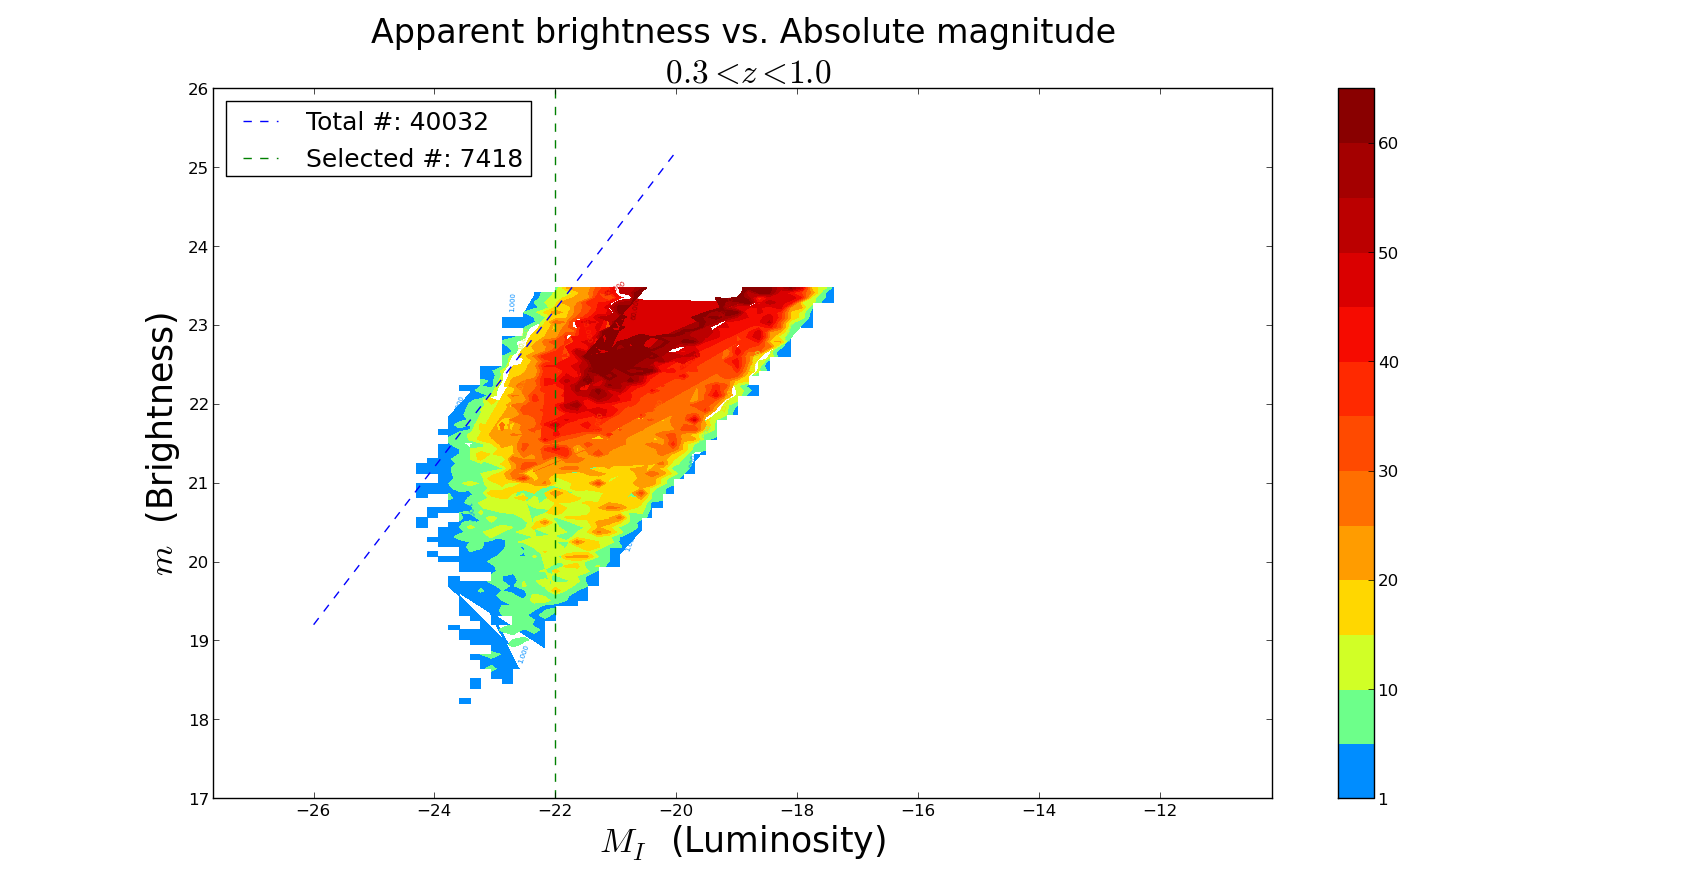
\includegraphics[width=\columnwidth]{Figures/fig1}
%   \label{fig:fig1}
%   \caption{}
% \end{figure}
% 
% {\bf Fig 2 - Histograms with diff MAG\_AUTO cuts}

\section{Modeling the redshift distribution}
\label{S:modelling}
With the above cut, we assign values for overdensity by fitting a parametric model to the histogram of photometric redshifts. This one-dimensional density is justified because the 
area we are considering is small for $z<1$. {\bf ?}. The figures show chi-squared and gamma functions fitted to the histogram. {\bf Motivation for these functional forms?}
For low $z$, the volume becomes too small to rely the overdensity values from our model fits and hence not considered. 
The curves are normalized such that the area under the curves is same as the number of galaxies considered.
{\bf Fig 3 - Histogram with fits }. \\
\begin{figure}[H]
 \centering
  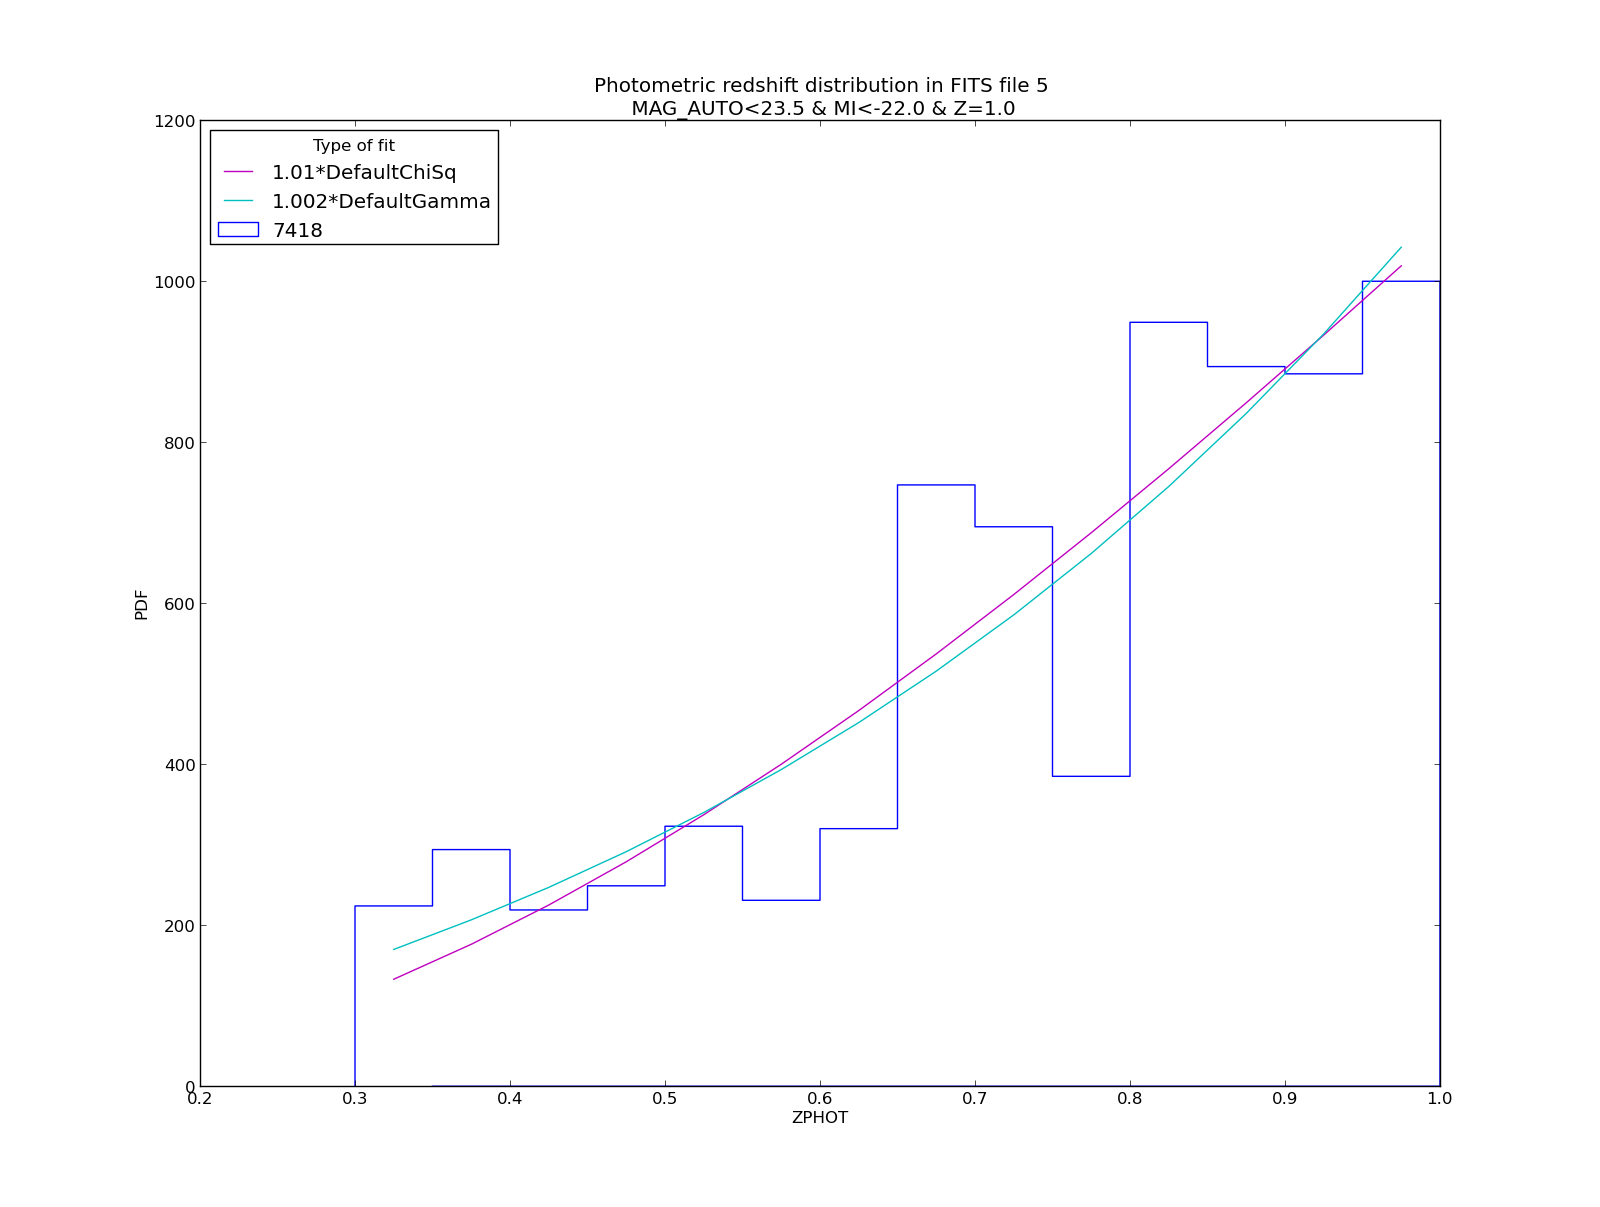
\includegraphics[width=\columnwidth]{Figures/fig3}
  \label{fig:fig3}
  \caption{}
\end{figure}

Overdensity in a redshift bin is defined as the ratio between the actual bin height and the value of the model. $\delta = N / N_{mod}$.
If $\delta$ from both the fits is greater than $1.1$, then we call that redshift bin as an
overdense region whereas if $\delta$ from both the fits is less than $0.9$, then we call that as an underdense region. {\bf Fig 4 - overdensities vs redshift bins}.

\begin{figure}
 \centering
 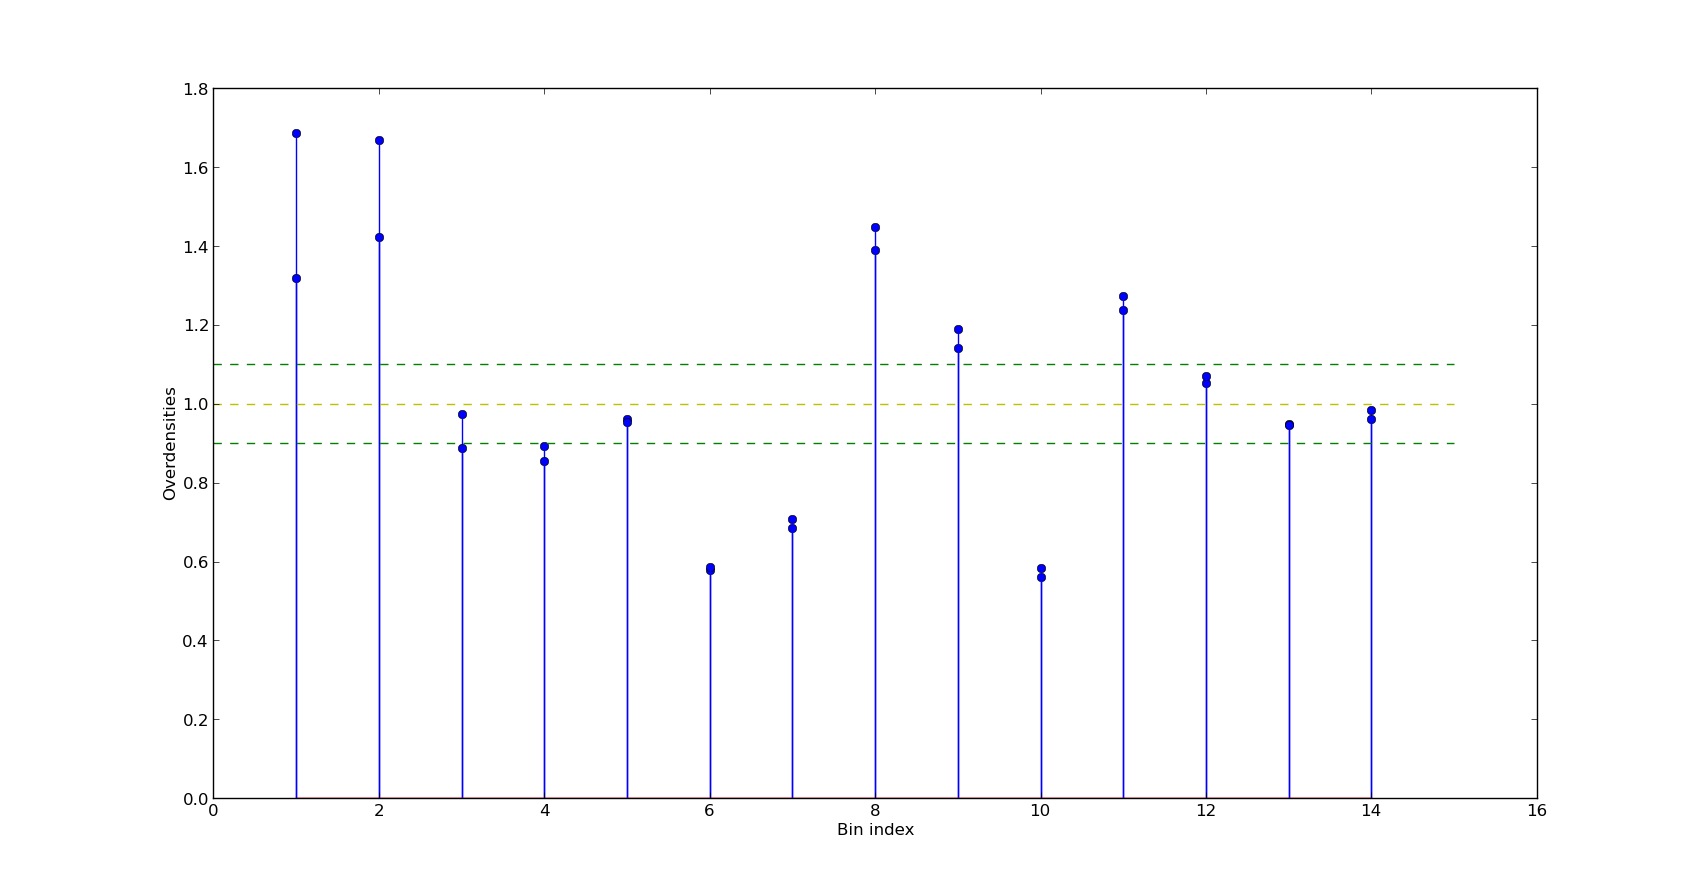
\includegraphics[width=\columnwidth]{Figures/fig4}
 \label{fig:fig4}
 \caption{}
\end{figure}

We see that the region between $0.85<z<1.0$ is neither overdense nor underdense according to our model and hence is not going to be considered for further analysis.
We use this to relax our luminosity cut to $-20.8$ so that the sample is still volume-limited for $z<0.85$. One can also convince oneself that such an assignment of overdensities
is sensible/robust by comparing the local mean co-moving density to the global mean co-moving density.

\begin{figure}
 \centering
 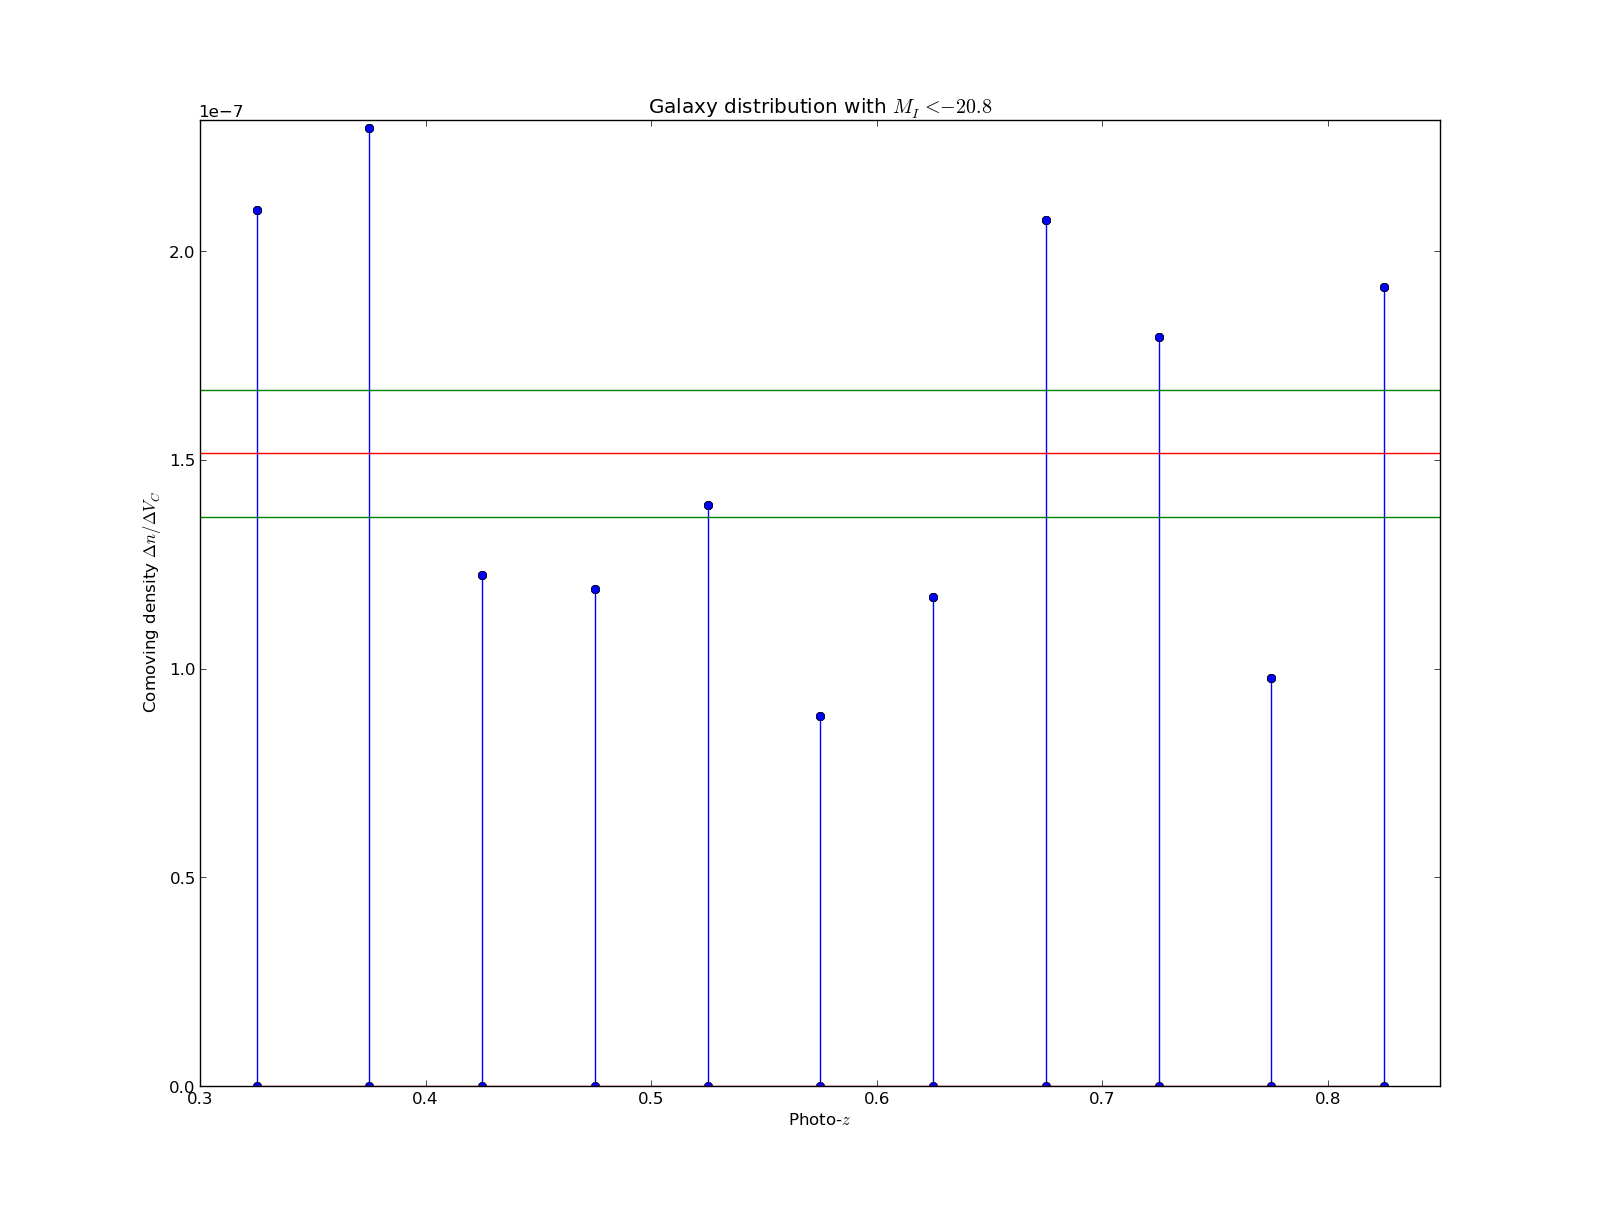
\includegraphics[width=\columnwidth]{../plots_20140219/comoving_densities(2b).png}
 \label{fig:comoving_densities}
 \caption{}
\end{figure}

In the following section, we will compare and analyze the distribution of properties of the galaxies residing in the overdense regions.

%
%\subsection{Correcting for SNR} 
%{\bf Fig 5 - hist\_magauto }. As seen in Fig 5, the overdense and the underdense regions differ in their brightness distributions. This translates to the overdense and the underdense regions 
%having different Signal-to-Noise ratios (SNR) and we need to correct for it. The fits are better for brighter galaxies and not as good for fainter ones. And there is a higher
%fraction of fainter galaxies in the underdense regions than in the overdense regions. To avoid any bias creeping in due to this, weights are assigned
%to the galaxies in the underdense regions such that
%the distributions of the brightness (MAG\_AUTO) scale to become identical. All other histograms that follow in this section are weighted.

\emph{Talk more about environments - Nature and nurture?}

\section{Implications/Comparisons}

\subsection{Comparison plots}
{\bf Insert Fig 6 - All histograms}

Quantitative results of this comparison is presented in {\bf Table 1}. Test statistic and $p$-values are obtained from Kolmogorov-Smirnov test (KS-test)
and 2-sample Anderson-Darlington tests (AD-test) are given below

%\begin{enumerate}
% \item KS2 - Kolmogorov-Smirnov 2 sample test on unweighted samples.
% \item ADK2 - Anderson Darlington K sample test on unweighted samples.
% \item KS - Kolmogorov-Smirnov test between the underdense sample and linearly-interpolated empirical CDF of the overdense sample weighted appropriately.
% \item KS2\_recon - Kolmogorov-Smirnov 2 sample test between the underdense sample and a sample drawn from the above mentioned CDF.
% \item ADK2\_recon - Anderson Darlington K sample test between the underdense sample and a sample drawn from the above mentioned CDF.  
%\end{enumerate}

{\bf Table 1 } - $p$-value matrix 
\begin{tabular}{||c|c|c||}
 \hline
  Field & KS p-value & AD p-value \\
 \hline 
  Apparent magnitude (m) & 1.972e-86 & 0.0 \\
  $i$-band Luminosity (\mi) & 1.459e-2 & 4.98e-3 \\
  Axis ratio $(b/a)$ & 4.277e-4 & 1e-4\\
  \sersicn & 1.593e-5 & 2e-5\\
  Color $(M_G-M_I)$ & 2.889e-2 & 7.8e-4\\
  
\end{tabular}

Having a conventional threshold for $p$-value $p_{threshold} = 0.05$, we conclude that the distributions are inconsistent from the above table.
When two randomly partitions of the sample is compared, the distributions are consistent with each other most of the time. The reason why the distributions
do not agree might partly because of the environment and partly because of the evolution with redshift. The subsequent sections are dedicated to separate out
their contributions.

%Average values of quantities of interest are plotted in {\bf Table 2}

%{\bf Table 2 } - Average values.

% \section{Redshift evolution}
% 
% Although randomly partitioned overdense galaxies were in agreement with each other,
% overdense regions at low redshifts are found to be incompatible with the overdense regions at higher redshifts.
% This suggests there could be 

\section{Axis ratio $(b/a)$}


{\bf to be transferred from the iPython notebook document}

\end{document}
